\documentclass[12pt]{scrbook}
\usepackage[utf8]{inputenc}
\usepackage{amsmath}
\usepackage{amsthm} %Para definir ambientes con \newtheorem
\usepackage{amsfonts}
\usepackage{amssymb}
\usepackage{makeidx}
\usepackage{graphicx}
\usepackage{natbib}
%\usepackage{float}

\title{Aprendizaje automático de reglas para operar en los mercados accionarios}
\publishers{Centro de Investigación en Computación, Instituto Politécnico Nacional}
\date{}
\author{David Ricardo Montalván Hernández}

%=========Define los ambientes a utilizar =======%
%Define estilo para dar un salto de línea en el encabezado
%del 'teorema'
\newtheoremstyle{break}
{2ex} %above space
{2ex} %below space
{\itshape} %Body font)
{} %indent amount
{\bfseries} %head font
{:} %post head puncuation
{\newline} %post head space
{}

\theoremstyle{break}
%Definición
\newtheorem{definicion}{Definicion}[chapter]

%Teorema
\newtheorem{teorema}{Teorema}[chapter]

%Algoritmo (Utiliza el ambiente tabbing)
\theoremstyle{break}
\newtheorem{algoritmo}{Algoritmo}[chapter]
%=================================================%

%====================Macros=======================%
\newcommand{\buyhold}{\textit{buy-and-hold}}
%=================================================%

\begin{document}
\maketitle
\pagenumbering{Roman} %numeración romana con mayúsculas
\renewcommand{\contentsname}{Contenido}
\tableofcontents
\renewcommand{\listfigurename}{Lista de imágenes}
\listoffigures
\renewcommand{\listtablename}{Lista de tablas}
\renewcommand\tablename{Tabla}
\renewcommand{\bibname}{Referencias}
\renewcommand{\figurename}{Imagen}
\listoftables

\chapter*{Dedicatoria}
A mis padres y amigos, quienes seguramente se reirán de esta dedicatoria y su "gran emotividad".

\chapter*{Agradecimientos}
Agradezco a mi director de tesis el doctor Salvador Godoy Calderón por enseñarme el enfoque simbólico del aprendizaje de máquina y por tener la paciencia suficiente para  intentar librarme (desafortunadamente sin éxito) de mis "manías estadísticas".

Agradezco también a cada uno de los miembros de mi comité tutorial por sus valiosas observaciones.

\chapter*{Resumen}
\chapter*{Abstract}

\pagenumbering{arabic} %Numeración árabe

%=============== INTRODUCCIÓN ================= %
\chapter{Introducción}
\label{capitulo:introduccion}
%Motivación y ¿qué es lo que se busca con este trabajo?
%Objetivo general y objetivos particulares.
%Estructura del trabajo.
El incremento en el poder de cómputo, la digitalización de los mercados financieros (en particular el mercado accionario) y la oportunidad de ganar dinero, son algunos de los factores que han motivado la investigación y desarrollo de algoritmos computacionales enfocados a guiar la toma de decisiones de inversión, en particular, determinar los momentos adecuados para realizar compras o ventas.

A pesar de que la idea básica es comprar barato y vender caro, la incertidumbre y complejidad de los mercados financieros han dado lugar al uso de herramientas computacionales con el fin de guiar la toma de decisiones, concretamente, técnicas relacionadas a la inteligencia artificial han ganado notoriedad.

El objetivo general de este trabajo es proponer una metodología para aprender, de manera automática, un conjunto de reglas \textit{IF..THEN}. Estas reglas se utilizarán para obtener estrategias de inversión cuya ganancia, buscamos, sea superior a la ganancia generada por la estrategia de \textbf{compra y espera} (ver sección \ref{seccion:hipotesis mercado eficiente}).

Una de las contribuciones de este trabajo es el análisis del mercado accionario mexicano, el cual está representado por el instrumento llamado \textbf{NAFTRAC ISHRS} (ver sección \ref{seccion:naftrac}).

Además, la metodología propuesta busca obtener un modelo interpretable, contrastando con la tendencia actual que se caracteriza por el uso de las llamadas \textit{cajas negras}, e.g., redes neuronales (ver capítulo \ref{capitulo:antecedentes}).

Los objetivos particulares de este trabajo son:
\begin{itemize}
\item Selección de atributos.

\item Etiquetado de datos.
\end{itemize}




%=============== Antecedentes ================= %
\chapter{Antecedentes}
\label{capitulo:antecedentes}
\begin{itemize}
\item Explicación de los artículos (en forma cronológica).
\end{itemize}

%=============== Marco teórico ================= %
\chapter{Marco teórico}
\label{capitulo:marco teorico}

\section{Mecánica de un mercado accionario}
\label{seccion:mecanica del mercado}

\section{Hipótesis del mercado eficiente}
\label{seccion:hipotesis mercado eficiente}

\section{NAFTRAC}
\label{seccion:naftrac}

\section{SPDR S\&P 500}
\label{seccion:sp500}

\section{Análisis técnico}
\label{seccion:analisisTecnico}



%=============== AQ y CN2 ================= %
\section{Algoritmos AQ y CN2}
\label{seccion:algoritmos aq cn2}

\subsection{Algoritmo AQ}
\label{subseccion:algoritmo aq}
El algoritmo quasi-óptimo (AQ), is un algoritmo de aprendizaje supervisado, que induce un conjunto de reglas del tipo \textit{IF-THEN} (ver \cite{AQCervone2010}, \cite{AQMichalski1991} y \cite{AQWojtusiak2012} para un estudio detallado). 

Dado un conjunto, $P$, con $n$ observaciones, $P_1, P_2, \ldots, P_n$ (ejemplos de la clase positiva)  y un conjunto, $N$, con $m$ observaciones, $Q_1, Q_2, \ldots, Q_m$ (ejemplos de la clase negativa), el algoritmo AQ encuentra un conjunto de reglas que son completas (cubren todos los ejemplos de la clase positiva) y consistentes (no cubren ejemplos de la clase negativa).

Las reglas toman la forma descrita en ecuación (\ref{eqn:reglas AQ})

\begin{equation} \label{eqn:reglas AQ}
Premisa \rightarrow Consecuente
\end{equation}

en donde $Premisa$ es una conjunción de condiciones (esta conjunción recibe el nombre de complejo) y cada condición tiene la estructura dada en la ecuación 

\begin{equation} \label{eqn:condicion AQ}
\left[Atributo\,\, OP\,\, Valores \right]
\end{equation}

en donde el término $OP$ depende del tipo de atributo que se está utilizando, por ejemplo, para un atributo con valores continuos tenemos que $OP \in \{>, \geq, <, \leq\}$.

El $Consecuente$ en (\ref{eqn:reglas AQ}), es una sola condición, por ejemplo, comprar.

El algoritmo AQ inicia su proceso de inducción seleccionando un ejemplo (semilla), $e$, de la clase positiva, el cual es generalizado creando todos los complejos que cubren $e$ y que son consistentes, es decir, que no cubren ningún ejemplo de la clase negativa. Este conjunto de complejos, $G(e,N)$, recibe el nombre de estrella. El mejor complejo en la estrella es seleccionado de acuerdo a un criterio previamente establecido, en este trabajo el criterio utilizado es maximizar el número de ejemplos positivos cubiertos. Este proceso es repetido hasta tener una disyunción de complejos que es completa y consistente, el algoritmo \ref{algo:AQ}

\begin{algoritmo}[Algoritmo AQ]
\begin{tabbing}
\\Sea $P$ el conjunto de ejemplos positivos de la clase C
\\Sea $N$ el conjunto de ejemplos negativos de la clase C\\
1. \=$Cobertura\leftarrow \emptyset $ \\
2. Mientras $P \neq \emptyset$:\\
 \>3. Elige semilla $e$ en $P$\\
 \>4. Genera estrella $G(e,N)$\\
 \>5. Selecciona el mejor complejo, $c$, en $G(e,N)$\\
 \>6. Agrega $c$ a $Cobertura$\\
 \>7. Elimina de $P$ los ejemplos cubiertos por $c$\\
\=8. Regresa $Cobertura$
\end{tabbing}
\label{algo:AQ}
\end{algoritmo}

\subsection{Algoritmo CN2}
\label{subseccion:algoritmo cn2}

\subsection{Soporte y exactitud de Laplace}
\label{subsec:Soport y exactitud de laplace}

%=============== Solución propuesta ================= %
\chapter{Solución propuesta}
\label{capitulo:solucion propuesta}

\section{Separación de datos}
\label{seccion:separacion de datos}
En este trabajo se utilizan precios diarios\footnote{Obtenidos de Yahoo Finance. https://finance.yahoo.com} de los instrumentos NAFTRAC y SPDR S\&P 500 (ver secciones \ref{seccion:naftrac} y \ref{seccion:sp500}).

Para el NAFTRAC, la información inicia el día 15 de febrero de 2013 y termina el 21 de enero de 2019. Para el SPDR S\&P 500 el periodo de tiempo abarcado es del 2 de enero de 2008 hasta  el 3 de marzo de 2019.

La tabla \ref{tabla:Ejemplo datos diarios NAFTRAC} muestra la estructura de los datos para el NAFTRAC, es importante señalar que los datos no incluyen días festivos ni fines de semana.

\begin{table}[h]
\centering
\begin{tabular}{cccccccc}
\hline
\textbf{Fecha} & \textbf{Apertura} & \textbf{Máximo} & \textbf{Mínimo} & \textbf{Cierre} & \textbf{Cierre ajustado} & \textbf{Volumen} \\
\hline
2013/02/15 & 44.09 & 44.24 & 43.86 & 44.18 & 41.61 & 77,614,608\\
2013/02/18 & 44.38 & 44.38 & 44.04 & 44.16 & 41.60 & 6,457,428\\
2013/02/19 & 44.34 & 44.77 & 44.29 & 44.63 & 42.05 & 68,042,072\\
\vdots & \vdots & \vdots & \vdots & \vdots & \vdots & \vdots \\
\hline
\end{tabular}
\caption{\label{tabla:Ejemplo datos diarios NAFTRAC} Datos diarios NAFTRAC}
\end{table}

Para crear nuestros conjuntos de entrenamiento y prueba, los datos se dividen utilizando una ventana deslizante de 90 días. Este criterio está fundamentado en el hecho de que, tanto en México como en Estados Unidos, las empresas con acciones listadas en alguna bolsa de valores, están obligadas a reportar los resultados de sus operaciones de manera trimestral, así pues, buscamos capturar la reacción de los inversionistas ante la publicación de dicha información.

La tabla \ref{tabla:data split SP500} muestra la separación de los datos del SPDR S\&P 500.
\begin{table}[h]
\centering
\begin{tabular}{cc}
\hline
\textbf{Entrenamiento} & \textbf{Prueba} \\
\hline
2008/01/02 - 2008/05/09 & 2008/05/12 - 2008/09/17 \\
2008/05/12 - 2008/09/17 & 2008/09/18 - 2009/01/27 \\
2008/09/18 - 2009/01/27 & 2009/01/28 - 2009/06/05 \\
\vdots & \vdots \\
\hline
\end{tabular}
\caption{\label{tabla:data split SP500} Separación de datos}
\end{table}

Observemos que con esta forma de separar los datos, un conjunto de prueba se convierte en un nuevo conjunto de entrenamiento, esto nos permite capturar el comportamiento dinámico de los mercados, en particular, su comportamiento no estacionario.

Utilizando esta metodología, se obtienen 15 conjuntos de entrenamiento y 15 conjuntos de prueba con la información del NAFTRAC, por otra parte, con los datos del SPDR S\&P 500 se obtienen 30 conjuntos de entrenamiento y 30 conjuntos de prueba.



\section{Proceso de etiquetado}
\label{seccion:proceso etiquetado}
Ya que nuestros datos de entrenamiento no están etiquetados, utilizamos un algoritmo evolutivo para obtener un conjunto de etiquetas que nos permita entrenar cada modelo. La idea detrás del etiquetado se basa en encontrar las combinaciones de compras y ventas que nos generen la mayor ganancia una vez conocida toda la historia del periodo de entrenamiento.

Este algoritmo evolutivo pertenece a la clase de algoritmos para la estimación de distribución (EDA por sus siglas en inglés \cite{simon2013evolutionary}). Cada individuo en la población representa una estrategia de inversión para un periodo de entrenamiento dado. Esta estrategia está representada a través de un vector $\mathbf{x} = (x_1, x_2, \ldots, x_t)$ cuya componente $x_i$ representan la acción a tomar en el día $i$, $x_i \in \{-1,0,1\}$, en donde $-1$ representa una señal de venta, $0$ una señal de espera y $1$ una señal de compra. La función de aptitud utilizada fue el exceso de ganancia sobre la estrategia \buyhold.

En la imagen \ref{imagen:etiquetado} vemos el resultado del proceso de etiquetado para un conjunto de entrenamiento en particular.

\begin{figure}[ht]
\centering
\scalebox{0.8}{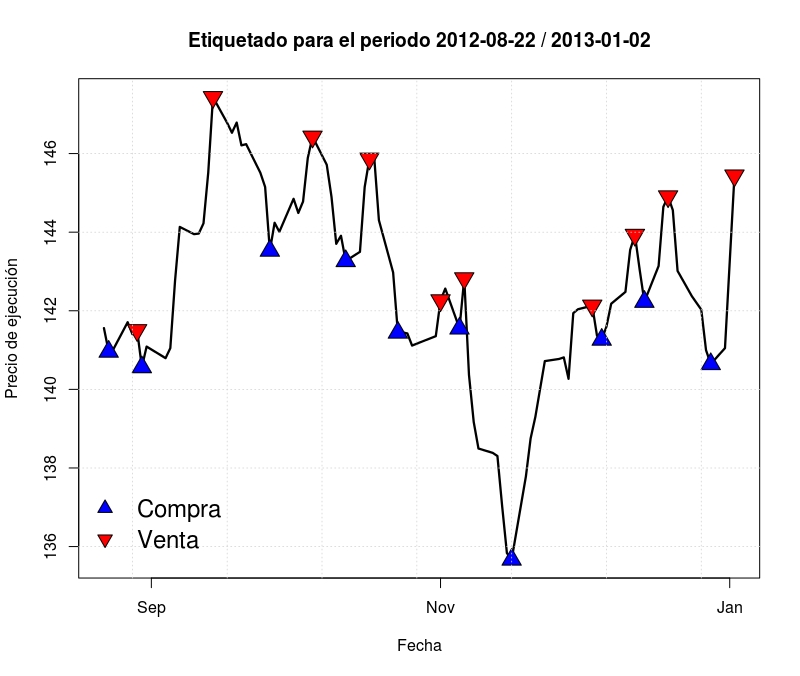
\includegraphics[width=1\linewidth]{imagenes/etiquetado.jpeg}}
\caption{\label{imagen:etiquetado} Resultado del proceso de etiquetado}
\end{figure}

\section{Atributos utilizados}
\label{seccion:atributos}
Los atributos utilizados en cada uno de los experimentos, son un conjunto de indicadores técnicos financieros (ver sección \ref{seccion:analisisTecnico}). Utilizamos estos indicadores ya que en ellos se refleja el conocimiento de los expertos, así como patrones que han demostrado ser útiles en la práctica.

Los indicadores utilizados son:
\begin{itemize}
\item Oscilador Aroon con una ventana de tiempo de 25 días para cada cada indicador Aroon.

\item RSI con una ventana de tiempo de 14 días.

\item MFI con una ventana de tiempo de 14 días.

\item Williams \%R con una ventana de tiempo de 14 días.

\item CCI con una ventana de tiempo de 20 días y un factor $C=0.015$.
\end{itemize}


\section{Aprendizaje incremental}
\label{seccion:aprendizaje incremental}
Tanto como para el algoritmo AQ como para el algoritmo CN2 se realizaron dos tipos de experimentos. El primero de ellos está basado en un enfoque de \textit{aprender-aplicar-descartar}, en el cual, dado un conjunto de entrenamiento, se induce un conjunto de reglas las cuales se aplican al conjunto de prueba más cercano. Después de esto, las reglas aprendidas se descartan (mecanismo de olvido).

El otro experimento se basa en un \textit{aprendizaje incremental}, en este caso aprendemos un conjunto de reglas y en lugar de descartarlas, las ordenamos de acuerdo a su desempeño sobre el conjunto de entrenamiento del cual fueron inducidas por primera vez, así como su desempeño sobre los conjuntos de prueba en los cuales han sido aplicadas. En este enfoque mantenemos un conjunto de $k$-mejores reglas de compra y $k$-mejores reglas de venta.

Para medir el desempeño de las reglas sobre los conjuntos de entrenamiento de los cuales se inducen por primera vez, utilizamos la suma de su \textit{soporte} y su \textit{exactitud de Laplace}.

En cambio, para medir el desempeño de las reglas sobre los conjuntos de prueba, las agrupamos en pares de \textit{compra-venta}. Estos pares de reglas se forman a partir de las señales de compra y venta generadas durante el periodo de prueba y son recompensadas (penalizadas) de acuerdo a la ganancia (pérdida) que generan.

Por ejemplo, consideremos un caso en el cual la regla de compra, $R_{C}$, nos indica que en el tiempo $t_1$ se debe de comprar, esta compra tendrá un precio de ejecución $P_{C}$. Conforme avanza el tiempo, notamos que la regla de venta, $R_{V}$, nos indica que en el tiempo $t_2 > t_1$, se debe de vender, esta venta tendrá precio de ejecución $P_{V}$. La recompensa (penalización) que se le asigna a cada regla en el par $\left(R_C, R_V\right)$ está dada por su ganancia (pérdida) porcentual, es decir:

\begin{equation}\label{eqn:recompensa reglas}
Recompensa(R_C, R_V) = \dfrac{P_V (1 - c)}{P_C (1 + c) } - 1
\end{equation}

en donde $c$ es el costo de transacción.

Finalmente, cada regla que no aparece en el conjunto de prueba que se está evaluando, se penaliza con la pérdida promedio que se tiene sobre este mismo conjunto de prueba; esto se utiliza como un mecanismo para ir descartando reglas debido al paso del tiempo.

De acuerdo a lo anterior, el puntaje de una regla $R$, antes de evaluar el conjunto de prueba $M$, está dado por:

\begin{equation} \label{eqn:puntaje de una regla}
puntaje_{-M}(R) = soporte(R) + Laplace(R) + \sum Recompensas
\end{equation}

en la ecuación (\ref{eqn:puntaje de una regla}), el término $ \sum Recompensas$ hace referencia a la suma de recompensas o penalizaciones que ha obtenido la regla $R$ para cada conjunto de prueba anterior al conjunto $M$.

De esta manera, ahora somos capaces de ordenar las reglas y por lo tanto acumular el aprendizaje así como identificar reglas útiles y descartar aquellas que no han funcionado.

La imagen \ref{imagen:aprendizaje_incremental} muestra el esquema del aprendizaje incremental que se propone en este trabajo.


\begin{figure}[ht]
\centering
\scalebox{1.0}{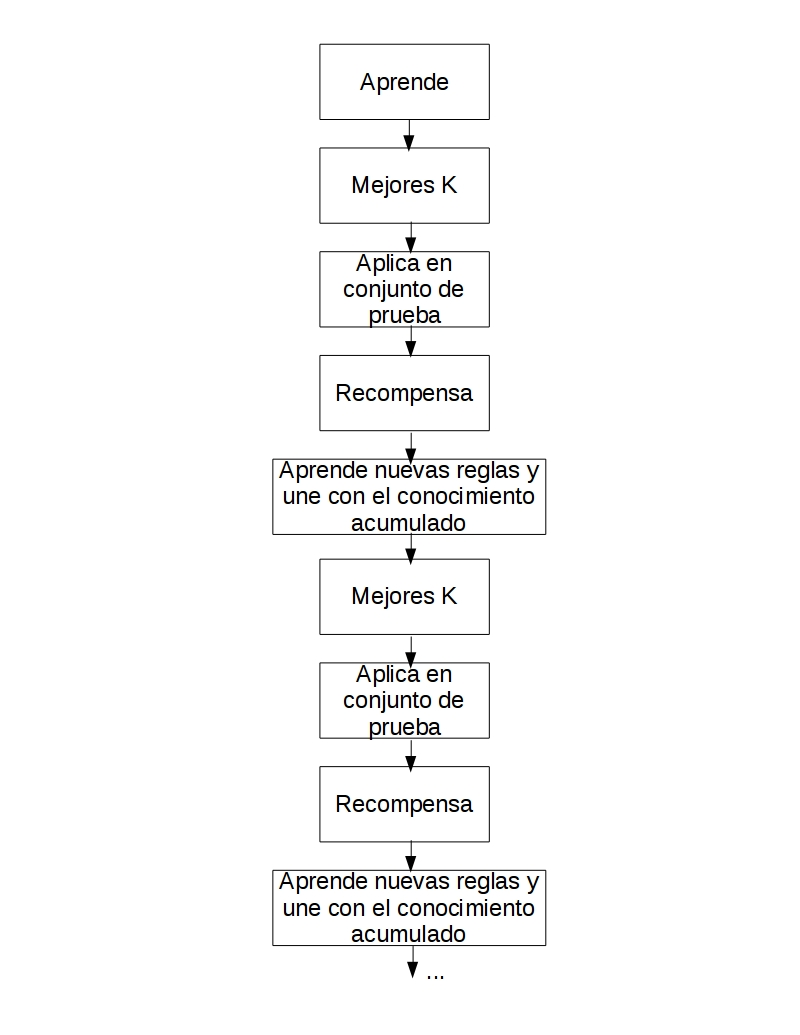
\includegraphics[width=1\linewidth]{imagenes/aprendizaje-incremental.jpg}}
\caption{\label{imagen:aprendizaje_incremental} Aprendizaje incremental}
\end{figure}


\section{Límites para las señales de venta}
\label{seccion:limites ventas}
Además de las reglas inducidas por cada algoritmo, utilizamos dos reglas adicionales las cuales buscan capturar el perfil de riesgo de los inversionistas.

Estas nuevas reglas establecen un límite superior (mercados a la alza) y un límite inferior (mercados a la baja) relativos a la última compra realizada. El primero de estos límites (límite superior) puede ser interpretado como el nivel de codicia que tiene un inversionista, mientras que el segundo (límite inferior) se interpreta como el nivel de aversión al riesgo.

De esta manera, se recibe una señal de venta en el tiempo $t$ si alguna de las siguientes condiciones se cumple:

\begin{align}
R_{venta} \wedge (Var_{t} > LS) \label{eqn:Venta limite sup}\\
R_{venta} \wedge (Var_{t} < LI) \label{eqn:Venta limite inf}
\end{align}

en donde $R_{venta}$ representa una regla de venta inducida por los algoritmos AQ o CN2, $LS$ es el límite superior expresado como un porcentaje relativo al último precio de compra, $LI$ es el límite inferior expresado como un porcentaje relativo al último precio de compra y $Var_{t}$ representa la variación porcentual del precio de ejecución en el tiempo $t$, $P_{t}^{ejec}$, respecto al último precio de compra, $P_{C}^{ult}$, como se muestra en la ecuación (\ref{eqn:variacion bandas})

\begin{equation} \label{eqn:variacion bandas}
Var_{t} = \dfrac{P_{t}^{ejec}}{P_{C}^{ult}} - 1
\end{equation}

La imagen \ref{imagen:bandas horizontales} muestra un ejemplo de los límites relativos a una señal de compra.

\begin{figure}[ht]
\centering
\scalebox{0.66}{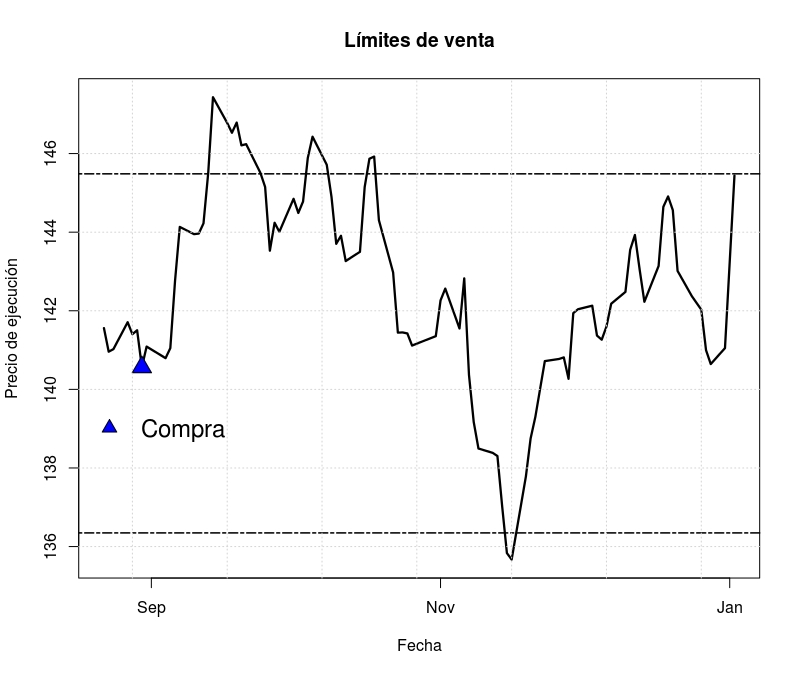
\includegraphics[width=1\linewidth]{imagenes/bandas_horizontales.jpeg}}
\caption{\label{imagen:bandas horizontales} Límites para las señales de venta relativos a una señal de compra}
\end{figure}

\section{Supuestos del mercado}
\label{sec:supuestos del mercado}
Para cada experimento, se consideraron los siguientes supuestos:

\begin{itemize}
\item El precio de ejecución en el día $t$ será el promedio entre el precio máximo y el precio mínimo de ese día.

\item Dada una señal de compra o venta en el día $t$, la acción se ejecuta en el día $t+1$ utilizando el precio de ejecución.

\item El costo de cada transacción se fija en $0.25\%$. Así para cada compra con precio de ejecución $P_{C}$ terminamos pagando un total de 
$$P_{C}(1 + 0.0025)$$
por cada acción comprada.

De la misma forma, por cada acción que vendemos a un precio $P_{V}$, recibimos 
$$P_{V}(1 - 0.0025)$$

\item En cada señal de compra, compramos tantas acciones podamos comprar con nuestro capital disponible (considerando el costo de transacción).

\item Para cada señal de venta, vendemos todas las acciones que poseamos.

\item Sólo podemos vender cuando tenemos acciones en nuestra posesión, es decir, no se permiten ventas en corto.

\item El límite superior para las señales de venta, $LS$, se fija con un valor de $0.035$ o $3.5\%$ relativo al último precio de compra.

\item El límite inferior para las señales de venta, $LI$, se fija con un valor de $-0.03$ o $-3.0\%$ relativo al último precio de compra. 
\end{itemize}

%=============== Resultados ================= %
\chapter{Resultados experimentales}
\label{capitulo:resultados experimentales}

%=============== Conclusión ================= %
\chapter{Conclusiones y trabajo futuro}
\label{capitulo:conclusiones}

\section{Conclusiones}
\label{seccion:conclusiones}

\section{Trabajo futuro}
\label{seccion:trabajo futuro}


\bibliography{references}
\addcontentsline{toc}{chapter}{Referencias}
\bibliographystyle{plain}







\end{document}